\section{Experimental Results} \label{sec5}
\noindent
We have built an end-to-end tool in Python for code replacement attack detection.
The tool takes in a set of control loop descriptions, computes their intersection and 
implements the cycle detection step. The tool has been applied to a number of small 
examples of synthetic control applications and their variants. Due to the lack of standard open
source benchmarks in this domain, we have performed all our experiments on synthetic benchmarks of 
various representative sizes, varying the number of individual control loops, and the number of constituent states of each.
For each row, for a fixed number of automata, we took up the initial descriptions and created random attacks by modifying some of the components,
and carried out our analysis. As expected, our tool was able to flag out the
schedulability violation in each of the cases. 

\textcolor{red}{Table~\ref{table:nonlin} presents overall performance of our experiment. The table shows whether
the tool is able to detect the attack or not. We have depicted that the system was schedulable before the attack
, in other way if the system is schedulable our tool is able to detect that. Now if one of the participated components
get attcked the system will become nonschedulable. Our system can capture this attack while examining the schedulability of the system.
The table also shows the scalability of the tool. With the increment of  participated components the scheduling time will also increase.}


Column 2 mentions the number of control applications participating in the control application, 
while the next 2 columns show whether the tool is able to detect schedulability and the time taken to perform that.
Columns 5 and 6 shows the performance of the tool for detecting the attack.

\begin{table}[ht]
\caption{Performance of the tool before and after attack}
\centering
\begin{tabular}{|c | c | c | c | c | c|}
%\hline
\hline %inserts double horizontal lines
Case & No.           &  All safe?       & Scheduling   & All are       &Scheduling  \\       
     & of            &  (before   & time in      & safe? (after   &time in            \\  
     & automata      &  attack)        & secconds     & attack)      &seconds    \\
\hline
\hline
1 & 2 & YES & 0.00069 & NO & 0.00038\\

2 & 4  & YES & 0.00354 & NO &  0.00054 \\

3 & 6  & YES & 0.00661 & NO & 0.00920 \\

4 & 8 & YES &  0.02248 & NO & 0.00693 \\

5 & 10 & YES & 0.23043 & NO & 0.14550 \\

6 & 12 & YES & 0.69302 & NO & 0.67120 \\

7 & 14 & YES & 1.78644 & NO & 1.74657 \\

8 & 16 & YES & 4.08354 & NO & 3.90508 \\

\hline

\end{tabular}
\label{table:nonlin}

\end{table}

\begin{comment}
\noindent
We explain our problem statement with a small example. Fig\ref{state} presents three automatons $P,Q$ and $R$ representing three different control applications.
Each has one initial state and an acceptance state. The acceptance states are the bus accessing states
of the automaton. To check for schedulability, we first construct the concurrent composition (the intersection automaton) of the individual automatons, as shown in Fig \ref{state-transition1}. The product construction is a little different from the classical product of finite automatons, and will be explained in the following section. \\ 

\noindent
We now consider a code replacement attack take places on this system. The resulting automaton is depicted in Fig \ref{replaced}.
As a result of this attack, one of the control loops is changed, as a result of which, there is a change in the structure of the intersection automaton. Our schedulability assessment on the new product automaton fails. As we can see in Fig \ref{graph_replaced}, there are no cycles which satisfy our infinitary scheduling condition, thus schedulability is no longer guaranteed and we conclude that a code replacement attack has taken place.

\begin{figure}
\begin{center}
\includegraphics[width=50mm]{motivating_example_automata.pdf}
\end{center}
\vspace{-0.1in}
\caption{{\em Initial Control loops}}
\label{state}
\end{figure}

\begin{figure}
\begin{center}
\includegraphics[width= 75mm]{graph.eps}
\end{center}
%\vspace{-0.1in}
\caption{{\em Initial Intersection automaton}}
\label{state-transition1}
\end{figure}

\begin{figure}
\begin{center}
\includegraphics[width= 50mm]{replaced.pdf}
\end{center}
%\vspace{-0.1in}
\caption{{\em Modified control loops after a replacement attack}}
\label{replaced}
\end{figure}


\begin{figure}
\begin{center}
\includegraphics[width= 50mm]{graph_replaced.eps}
\end{center}
%\vspace{-0.1in}
\caption{{\em Intersection automaton after a code replacement attack}}
\label{graph_replaced}
\end{figure}
\end{comment}